\section{Unmanned Aerial Vehicle}\label{sec:design_uav}

For the \gls{uav} design, the following components are considered: the airframe, the propulsion system, the flight controller, the power system, and peripherals.

\subsection{Airframe}

The airframe is the structure of the \gls{uav} that holds all the components together. The airframe must be lightweight, durable, and easy to assemble and disassemble. The airframe must also be able to carry the peripherals and additional components required for the reconnaissance tasks.

For the airframe, different designes are considered, such as fixed-wing, rotary-wing, and hybrid designs as stated in \cref{sec:uav_types}. As on of the main requirements is the ability to take off and land in remote areas with limited infrastructure, a rotary-wing design is chosen for the \gls{uav}. The rotary-wing design allows for vertical takeoff and landing, as well as the ability to hover in place, which is useful for reconnaissance tasks.

Rotary-wing designs are further divided into multi-rotor and single-rotor designs as seen in \cref{fig:rotary_wing_designs}. Multi-rotor designs are more stable and easier to control, while single-rotor designs are more efficient and have a longer flight time. For the \gls{uav} design, a quadcopter design is chosen, as it provides a good balance between stability and efficiency.

\begin{figure}
  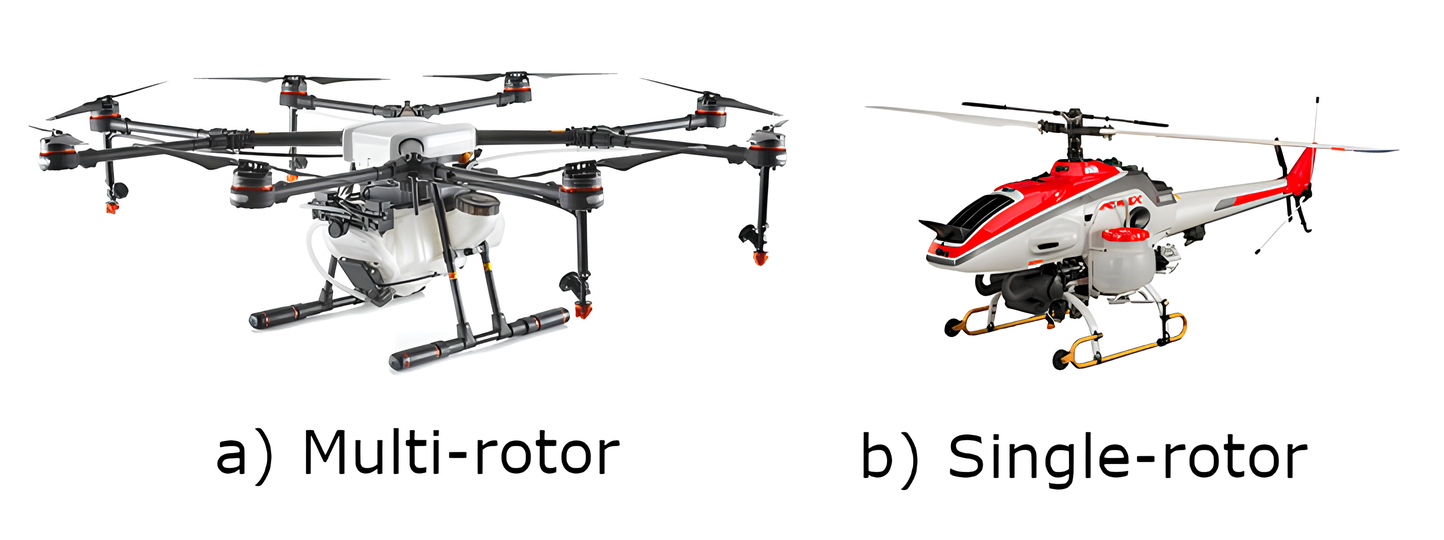
\includegraphics{rotary_wing_designs.png}
  \caption{Rotary-wing designs. Reproduced from \autocite{rotary_wing_designs}.
  }\label{fig:rotary_wing_designs}
\end{figure}

For the material of the airframe, a lightweight and durable material is chosen, such as carbon fiber or aluminum. The airframe is designed to be modular, allowing for the integration of different sensors and payloads for different applications. And finally, the airframe is designed to be cost-effective and commercially available, with the ability to be assembled and disassembled easily, and to be repaired and maintained with minimal effort.


For that case the airframe chosen \todo{add ref to where we bought it} is the \todo{add which one}. It is a quadcopter design made of carbon fiber, with a wingspan of \todo{add size} and a maximum takeoff weight of \todo{add weight}. The airframe is designed to carry a maximum payload weight of \todo{add weight}, with the ability to adapt to different reconnaissance tasks. Moreover, it has a payload bay that allows for the integration of different sensors and payloads, such as cameras, lidar, and thermal imaging sensors.

\todo{ add image of the aireframe chosen }

\subsection{Propulsion System}\label{subsec:design_propulsion_system}

The propulsion system is the system that provides the thrust required for the \gls{uav} to take off, land, and navigate. The propulsion system can be of different types, such as electric, gasoline, or hybrid. Electric propulsion systems are usually chosen for \glspl{uav} due to their efficiency, reliability, and low maintenance requirements. Gasoline propulsion systems are usually chosen for larger \glspl{uav} that require longer flight times and higher payloads. Hybrid propulsion systems are usually chosen for \glspl{uav} that require both efficiency and long flight times.

For the \gls{uav} design, an electric propulsion system is chosen, as it provides a good balance between efficiency, reliability, and low maintenance requirements. The electric propulsion system consists of four brushless motors, four electronic speed controllers, and four propellers. The main requirements of the propulsion system are the ability to provide enough thrust for the \gls{uav} to take off, land, and navigate, as well as the ability to carry the maximum payload weight of \todo{add weight}.

The brushless motors chosen were the \todo{add ref to where we bought them}, with a maximum thrust of \todo{add thrust} and a maximum power of \todo{add power}. The electronic speed controllers chosen were the \todo{add ref to where we bought them}, with a maximum current of \todo{add current} and a maximum voltage of \todo{add voltage}. The propellers chosen were the \todo{add ref to where we bought them}, with a maximum diameter of \todo{add diameter} and a maximum pitch of \todo{add pitch}. This complete propulsion system is designed to provide a thrust-to-weight ratio of \todo{add ratio}, with the ability to carry the maximum payload weight of \todo{add weight} which meets the requirements of the \gls{uav} design.

\todo{ add image of the propulsion system chosen }

\subsection{Flight Controller}

The flight controller is the system that controls the \gls{uav} during flight. The flight controller is responsible for stabilizing the \gls{uav}, controlling the motors, and navigating the \gls{uav} to a set of waypoints. The flight controller can be of different types, such as manual, semi-autonomous, or autonomous. Manual flight controllers are usually chosen for \glspl{uav} that require human intervention during flight. Semi-autonomous flight controllers are usually chosen for \glspl{uav} that require human intervention for takeoff and landing, but can navigate autonomously to a set of waypoints. Autonomous flight controllers are usually chosen for \glspl{uav} that can take off, land, and navigate autonomously to a set of waypoints. One key feature of the flight controller is the \textit{Return to Home} feature, which allows the \gls{uav} to return to the ground station in case of loss of communication or other critical failures.

For the \gls{uav} design, an autonomous flight controller is chosen, as it provides the ability to take off, land, and navigate autonomously to a set of waypoints. Commercially, there are multiple flight controllers available \todo{ref to table} and any of them can be used for the \gls{uav} design. The main requirements of the flight controller are the ability to stabilize the \gls{uav}, control the motors, and navigate the \gls{uav} to a set of waypoints, as well as the ability to communicate with the ground station in real-time. The flight controller chosen was the \todo{add ref to where we bought it}, as \todo{add reasons} An image of the flight controller is shown in \todo{add ref to fig}.

\todo{ add table of flight controllers }

\todo{ add image of the flight controller chosen }

\subsection{Power System}\label{subsec:design_power_system}

The power system is the system that provides the power required for the \gls{uav} to operate. The power system can be of different types, such as batteries, fuel cells, or solar panels. For \glspl{uav}, usually batteries are chosen, as they provide a good balance between energy density, power density, and weight. The main requirements of the power system are the ability to provide enough power for the \gls{uav} to take off, land, and navigate, as well as the ability to carry the maximum payload weight of \todo{add weight}.

For the \gls{uav} design, a lithium polymer battery is chosen, as it provides a good balance between energy density, power density, and weight. The battery chosen was the \todo{add ref to where we bought it}, with a maximum capacity of \todo{add capacity} and a maximum voltage of \todo{add voltage}. The battery is designed to provide enough power for the \gls{uav} to take off, land, and navigate, as well as the ability to carry the maximum payload weight of \todo{add weight}. The battery is also designed to be modular, allowing for the integration of different batteries for different applications.

\todo{ add image of the power system chosen }

Moreover, usually the power system is divided into two parts, the power distribution system for the propulsion system and the power management system for the electronics. The main reason for this distinction is that the propulsion system requires a high current and low voltage, while the electronics require a low current and high voltage. However, for the \gls{uav} design, the power system is integrated into a single system to reduce weight and complexity and specially the pricing of the system.

Futhermore, in order to provide the required power for the different components of the \gls{uav}, a power management system is integrated into the power system. The power management system consists of a battery monitor, a voltage regulator, and a current sensor. The one chosen was the \todo{add ref to where we bought it}, with a maximum current of \todo{add current} and a maximum voltage of \todo{add voltage}. The power management system is designed to provide the required power for the different components of the \gls{uav}, as well as the ability to monitor the battery voltage and current in real-time. And finally, a voltage regulator is integrated into the power system to provide the required voltage for the reconnaissance platform and the communication system. The voltage regulator chosen was the \todo{add ref to where we bought it}, with a maximum voltage of \todo{add voltage} and a maximum current of \todo{add current}. The voltage regulator is designed to provide the required voltage for the reconnaissance platform and the communication system, as well as the ability to monitor the voltage and current in real-time.

\todo{ add image of the power management system chosen }

\subsection{Peripherals}

The peripherals are the components that provide additional functionality to the \gls{uav}. The peripherals can be of different types, such as sensors, geo-location systems, cameras, lidar, or thermal imaging sensors. For reconnaissance tasks, usually sensors and cameras are chosen, as they provide the ability to collect data and images of the environment. The main requirements of the peripherals are the ability to collect data and images of the environment, as well as the ability to relay the information to the ground station in real-time.

For the \gls{uav} design, a \gls{gps} module was integrated into the \gls{uav}, as it provides the ability to navigate the \gls{uav} to a set of waypoints. The \gls{gps} module chosen was the \todo{add ref to where we bought it}, with a maximum accuracy of \todo{add accuracy} and a maximum update rate of \todo{add rate}. The \gls{gps} module is designed to provide the ability to navigate the \gls{uav} to a set of waypoints, as well as the ability to relay the information to the ground station in real-time. An image of the \gls{gps} module is shown in \todo{add ref to fig}.

\todo{ add image of the gps module chosen }

Moreover, a kill switch was integrated into the \gls{uav}, as it provides the ability to stop the motors in case of an emergency. It is a required safety feature for \glspl{uav} to prevent accidents and injuries. The kill switch chosen was the \todo{add ref to where we bought it}.

\todo{ add image of the kill switch chosen }

Finally, a camera was integrated into the \gls{uav}, as it provides the ability to collect images of the environment. The camera chosen was the \todo{add ref to where we bought it}, with a maximum resolution of \todo{add resolution} and a maximum frame rate of \todo{add rate}. The camera is designed to provide the ability to collect images of the environment, as well as the ability to relay the information to the ground station in real-time. An image of the camera is shown in \todo{add ref to fig}.

\todo{ add image of the camera chosen }

% Local Variables:
% jinx-local-words: "aireframe uav"
% End:
